\documentclass[sectionformat=excercise]{gadsescript}

\usetikzlibrary{shapes}

\setsemester{Winter Semester 2023/2024}%
\setuniversity{University of Konstanz}%
\setfaculty{Faculty of Science\\(Computer and Data Science)}%
\settitle{Elias Gestrich}
\setsubtitle{Finite state macines, regular languages}

\begin{document}
\maketitle
\section{Finite-State Machines, Regular Language}
\begin{enumerate}[label=\alph*)]
	\item $ M = ( \left\{ S, A, B \right\} , \left\{ a, b \right\} , \left\{ \delta(S, a) = B, \delta(S, b) = A, \delta(A, a) = A, \delta(A, b) = B, \delta(B, b) = A \right\} , S, A ) $
	\item SBAABA
\end{enumerate}

\section{Finite-State Machines II}
\begin{enumerate}[label=\alph*)]
	\item no
	\item yes
	\item ~\\
		\begin{tikzpicture}
                        \node[draw, circle, minimum size = 40] (a) at (0,0) {$ z_a $};
                        \node[draw, circle, minimum size = 40] (ab) at (4,0) {$ z_a z_b $};
                        \node[draw, circle, minimum size = 40] at (4,4) {$ z_a z_b z_c $};
                        \node[draw, circle, minimum size = 45] (abc) at (4,4) {};
                        \node[draw, circle, minimum size = 40] at (4,-4) {$ z_a z_c $};
                        \node[draw, circle, minimum size = 45] (ac) at (4,-4) {};
			\draw[-stealth] (-1.5, 0) -- (a);
			\draw[->] (a) to[out=120,in=60,loop] node[midway,above,inner sep=2pt] {1} ();
			\draw[-stealth] (a) -- node[midway, above] {0} (ab);
			\draw[-stealth] (ab) -- node[midway, left] {0} (abc);
			\draw[-stealth] (ab) to[out=-120, in=120] node[midway, left] {1} (ac);
			\draw[-stealth] (ac) to[out=60, in=-60] node[midway, right] {0} (ab);
			\draw[-stealth] (ac) -- node[midway, below left] {1} (a);
			\draw[-stealth] (abc) to[out=120, in=60, loop] node[midway, above] {0} (abc);
			\draw[-stealth] (abc) to[out=-30, in=30] node[midway, right] {1} (ac);
                \end{tikzpicture}
	\item $ (0|1)^*0(0|1) $
\end{enumerate}
\section{Type-3 Grammars}
\begin{enumerate}[label=\alph*)]
	\item no
		\setcounter{enumi}{2}
	\item $ M_3 = (\left\{ V_1, V_2, X \right\} , \left\{ a, b \right\} , \delta, V_2, X ) $ with\\
		\begin{tabular}{|c||c|c|}
			\hline
			$ \delta $ & $ a $ & $ b $ \\\hline
			$ V_1 $ & $ \left\{ X, V_1 \right\}  $ & $ X $ \\
			$ V_2 $ & $ V_1 $ & $ V_2 $ \\
			$ X $ &  & \\\hline
		\end{tabular}\\
		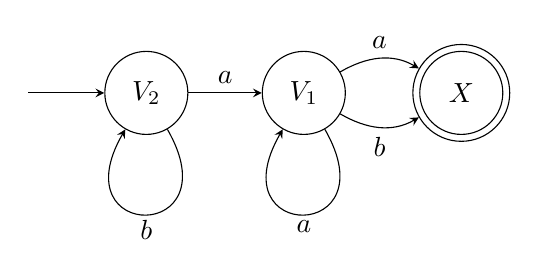
\begin{tikzpicture}
                        \node[draw, circle, minimum size = 30] (2) at (0,0) {$ V_2 $};
                        \node[draw, circle, minimum size = 30] (1) at (2,0) {$ V_1 $};
                        \node[draw, circle, minimum size = 30] at (4,0) {$ X $};
                        \node[draw, circle, minimum size = 35] (x) at (4,0) {};
			\draw[-stealth] (-1.5, 0) -- (2);
			\draw[-stealth] (2) to[out=-60,in=-120,loop] node[midway,below,inner sep=2pt] {$ b $} ();
			\draw[-stealth] (2) -- node[midway, above] {$ a $} (1);
			\draw[-stealth] (1) to[out=30, in=150] node[midway, above] {$ a $} (x);
			\draw[-stealth] (1) to[out=-60,in=-120,loop] node[midway,below,inner sep=2pt] {$ a $} ();
			\draw[-stealth] (1) to[out=-30, in=-150] node[midway, below] {$ b $} (x);
                \end{tikzpicture}
\end{enumerate}
\end{document}
